\section*{Aufgabe 1}
\subsection*{a)}
für m=1
\[
  \{1, 2, 3, 4\}
\]
für m=2
\begin{align*}
  &\{\{1\}\{2,3,4\}\},\{\{2\}\{1,3,4\}\},\{\{3\}\{1,2,4\}\},\{\{4\}\{1,2,3\}\},\{\{1,2\}\{3,4\}\}, \\
  &\{\{1,3\}\{2,4\}\},\{\{1,4\}\{2,3\}\}
\end{align*}
für m=3
\begin{align*}
  &\{\{1\}\{2\}\{3,4\}\},\{\{1\}\{3\}\{2,4\}\},\{\{2\}\{3\}\{1,4\}\},\{\{3\}\{4\}\{1,2\}\},\\
  &\{\{1\}\{4\}\{2,3\}\},\{\{2\}\{4\}\{1,3\}\}
\end{align*}
für m=4
\[
  \{\{1\}\{2\}\{3\}\{4\}\}
\]

\pagebreak
\subsection*{b)}
Wir zeigen, dass 
\[
  \sum_{m=0}^{n} S(n,m) = \sum_{k=0}^{n-1} \binom{n-1}{k}B_k = B_n
\]
Zuerst formen wir um
\[
  \sum_{m=0}^{n} S(n,m) = S(n,n) + \sum_{m=0}^{n-1} S(n,m) = 1 + \sum_{m=0}^{n-1} S(n,m)
\]
und verwenden Dann die Formel für die Stirlingzahlen aus Satz 1.9.10
\[
  1 + \sum_{m=0}^{n-1} S(n,m) = 1 + \sum_{m=0}^{n-1} \sum_{k=m}^{n-1} \binom{n-1}{k} S(k,m) .
\]
Nun lösen wir die Summen auf (Wir lassen die 1 am Anfang raus weil wir keine Ahnung haben wo wir sie in der Folgenden Form einbringen sollen)
\[
  \binom{n-1}{0}S(0,0) + \binom{n-1}{1}(S(1,0) + S(1,1)) + \ldots + \binom{n-1}{n-1}(S(n-1,0) + \ldots + S(n-1,n-1))
\]
Hier ist eine Visualisierung warum wir es so auflösen können \\
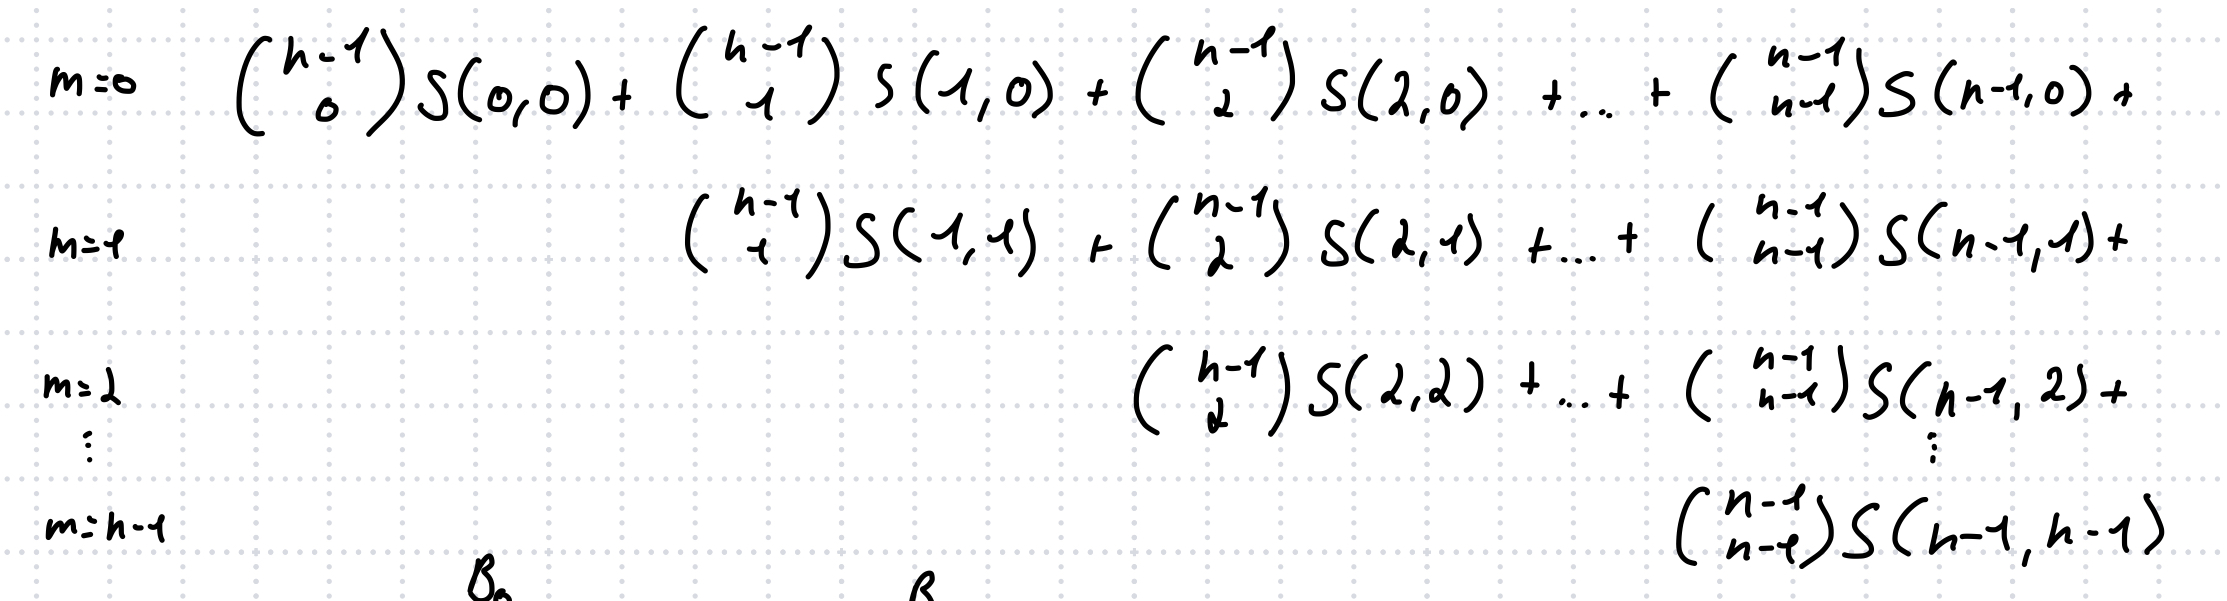
\includegraphics[width=\linewidth]{img/ex1.jpeg} \\
Dies können wir umformen zu
\[
  \sum_{k=0}^{n-1}\left(\binom{n-1}{k} \sum_{m=0}^{k}S(k,m)\right) = \sum_{k=0}^{n-1}\binom{n-1}{k} B_k
\]
Wodurch wir gezeigt haben, dass
\[
  \sum_{k=0}^{n-1} \binom{n-1}{k}B_k = B_n
\]

\subsection*{c)}
Anwenden der Formel $\sum_{k=0}^{i}\binom{i}{k}B_k$
\begin{align}
&B_0 = B_1 = 1 \\
&B_2 = B_0 + B_1 = 2 \\
&B_3 = B_0 + 2B_1 + B_2 = 5 \\
&B_4 = B_0 + 3B_1 + 3B_2 + B_3 = 15
\end{align}
Das Ergebnis beschreibt die Anzahl der Äquivalenzrelationen für $M=\{1,2,3,4\}$. Die Anzahl in a) stimmt mit dem Ergebnis aus c) überein.
